\documentclass{beamer}
\mode<presentation> {

%\usetheme{default}
\usetheme{Amsterdam}
%\usetheme{AnnArbor}
%\usetheme{Antibes}
%\usetheme{Bergen}
%\usetheme{Berkeley}
%\usetheme{Berlin}
%\usetheme{Boadilla}
%\usetheme{CambridgeUS}
%\usetheme{Copenhagen}
%\usetheme{Darmstadt}
%\usetheme{Dresden}
%\usetheme{Frankfurt}
%\usetheme{Goettingen}
%\usetheme{Hannover}
%\usetheme{Ilmenau}
%\usetheme{JuanLesPins}
%\usetheme{Luebeck}
%\usetheme{Madrid}
%\usetheme{Malmoe}
%\usetheme{Marburg}
%\usetheme{Montpellier}
%\usetheme{PaloAlto}
%\usetheme{Pittsburgh}
%\usetheme{Rochester}
%\usetheme{Singapore}
%\usetheme{Szeged}
%\usetheme{Warsaw}

% As well as themes, the Beamer class has a number of color themes
% for any slide theme. Uncomment each of these in turn to see how it
% changes the colors of your current slide theme.

%\usecolortheme{albatross}
%\usecolortheme{beaver}
%\usecolortheme{beetle}
%\usecolortheme{crane}
%\usecolortheme{dolphin}
%\usecolortheme{dove}
%\usecolortheme{fly}
%\usecolortheme{lily}
%\usecolortheme{orchid}
%\usecolortheme{rose}
%\usecolortheme{seagull}
%\usecolortheme{seahorse}
%\usecolortheme{whale}
%\usecolortheme{wolverine}

%\setbeamertemplate{footline} % To remove the footer line in all slides uncomment this line
%\setbeamertemplate{footline}[page number] % To replace the footer line in all slides with a simple slide count uncomment this line
\setbeamertemplate{navigation symbols}{}
}

\usepackage[utf8]{inputenc}

% INCLUYE LAS IMAGENES
\usepackage{graphicx}

% LIBRERIA PARA REGULAR POSICION DE TABS
\usepackage{booktabs}

% LIBRERIAS PARA CIRCUITOS
\usepackage{tikz}
\usetikzlibrary{matrix,calc,arrows}
\usetikzlibrary{positioning}
\usepackage{circuitikz}


\newcommand{\implicant}[3][0]{
    \draw[rounded corners=3pt] ($(#2.north west)+(135:#1)$) rectangle ($(#3.south east)+(-45:#1)$);
    }

%group lateral borders
%#1-space between node and grouping line. Default=0
%#2-top left node
%#3-bottom right node
\newcommand{\implicantcostats}[3][0]{
    \draw[rounded corners=3pt] ($(rf.east |- #2.north)+(90:#1)$)-| ($(#2.east)+(0:#1)$) |- ($(rf.east |- #3.south)+(-90:#1)$);
    \draw[rounded corners=3pt] ($(cf.west |- #2.north)+(90:#1)$) -| ($(#3.west)+(180:#1)$) |- ($(cf.west |- #3.south)+(-90:#1)$);
}

%group top-bottom borders
%#1-space between node and grouping line. Default=0
%#2-top left node
%#3-bottom right node
\newcommand{\implicantdaltbaix}[3][0]{
    \draw[rounded corners=3pt] ($(cf.south -| #2.west)+(180:#1)$) |- ($(#2.south)+(-90:#1)$) -| ($(cf.south -| #3.east)+(0:#1)$);
    \draw[rounded corners=3pt] ($(rf.north -| #2.west)+(180:#1)$) |- ($(#3.north)+(90:#1)$) -| ($(rf.north -| #3.east)+(0:#1)$);
}

%group corners
%#1-space between node and grouping line. Default=0
\newcommand{\implicantcantons}[1][0]{
    \draw[rounded corners=3pt] ($(rf.east |- 0.south)+(-90:#1)$) -| ($(0.east |- cf.south)+(0:#1)$);
    \draw[rounded corners=3pt] ($(rf.east |- 8.north)+(90:#1)$) -| ($(8.east |- rf.north)+(0:#1)$);
    \draw[rounded corners=3pt] ($(cf.west |- 2.south)+(-90:#1)$) -| ($(2.west |- cf.south)+(180:#1)$);
    \draw[rounded corners=3pt] ($(cf.west |- 10.north)+(90:#1)$) -| ($(10.west |- rf.north)+(180:#1)$);
}
\def\ol#1{\overline{#1}}
%Empty Karnaugh map 4x4
\newenvironment{Karnaugh}%
{
\begin{tikzpicture}[baseline=(current bounding box.north),scale=0.8]
\draw (0,0) grid (4,4);
%
\matrix (mapa) [matrix of nodes,
        column sep={0.8cm,between origins},
        row sep={0.8cm,between origins},
        every node/.style={minimum size=0.3mm},
        anchor=8.center,
        ampersand replacement=\&] at (0.5,0.5)
{
                       \& |(c00)| $\ol{yw}$  \& |(c01)| $\ol{y}w$  \& |(c11)| $yw$       \& |(c10)| $y\ol{w}$  \& |(cf)| \phantom{00} \\
|(r00)| $\ol{xz}$      \& |(0)|  \phantom{0} \& |(1)|  \phantom{0} \& |(3)|  \phantom{0} \& |(2)|  \phantom{0} \&                     \\
|(r01)| $\ol{x}z$      \& |(4)|  \phantom{0} \& |(5)|  \phantom{0} \& |(7)|  \phantom{0} \& |(6)|  \phantom{0} \&                     \\
|(r11)| $xz$           \& |(12)| \phantom{0} \& |(13)| \phantom{0} \& |(15)| \phantom{0} \& |(14)| \phantom{0} \&                     \\
|(r10)| $x\ol{z}$      \& |(8)|  \phantom{0} \& |(9)|  \phantom{0} \& |(11)| \phantom{0} \& |(10)| \phantom{0} \&                     \\
|(rf) | \phantom{00}   \&                    \&                    \&                    \&                    \&                     \\
};
}%
{
\end{tikzpicture}
}

%Empty Karnaugh map 2x4
\newenvironment{Karnaughvuit}%
{
\begin{tikzpicture}[baseline=(current bounding box.north),scale=0.8]
\draw (0,0) grid (4,2);
%
\matrix (mapa) [matrix of nodes,
        column sep={0.8cm,between origins},
        row sep={0.8cm,between origins},
        every node/.style={minimum size=0.3mm},
        anchor=4.center,
        ampersand replacement=\&] at (0.5,0.5)
{
                      \& |(c00)| $\ol{BA}$  \& |(c01)| $\ol{B}A$  \& |(c11)| $BA$       \& |(c10)| $B\ol{A}$  \& |(cf)| \phantom{00} \\
|(r00)| $\ol{C}$      \& |(0)|  \phantom{0} \& |(1)|  \phantom{0} \& |(3)|  \phantom{0} \& |(2)|  \phantom{0} \&                     \\
|(r01)| $C$           \& |(4)|  \phantom{0} \& |(5)|  \phantom{0} \& |(7)|  \phantom{0} \& |(6)|  \phantom{0} \&                     \\
|(rf) | \phantom{00}  \&                    \&                    \&                    \&                    \&                     \\
};
}%
{
\end{tikzpicture}
}

%Defines 8 or 16 values (0,1,X)
\newcommand{\contingut}[1]{%
\foreach \x [count=\xi from 0]  in {#1}
     \path (\xi) node {\x};
}

%Places 1 in listed positions
\newcommand{\minterms}[1]{%
    \foreach \x in {#1}
        \path (\x) node {1};
}

%Places 0 in listed positions
\newcommand{\maxterms}[1]{%
    \foreach \x in {#1}
        \path (\x) node {0};
}

%Places X in listed positions
\newcommand{\indeterminats}[1]{%
    \foreach \x in {#1}
        \path (\x) node {X};
}


%%%%%%%%%%%%%%%%%%%%%%%%%%%%%%%%%%%%%%%%%%%%%%%%%%%%%%%%%%%%%%%%%%%%%%%%%%%%%
%%%%%%%%	ACA VAN LAS DEFINICIONES PARA CIRCUITOS SECUENCIALES	 %%%%%%%%
%%%%%%%%%%%%%%%%%%%%%%%%%%%%%%%%%%%%%%%%%%%%%%%%%%%%%%%%%%%%%%%%%%%%%%%%%%%%%

\def\JKFF(#1)#2#3{%
  \begin{scope}[shift={(#1)}]
    \draw (0,0) rectangle (1,1);
    \draw (0.5,1) -- (0.5,0);
    \draw (0.5,0.5) -- (1,0.5);
    \node at (0.75,0.75) {$Q$};
    \node at (0.75,0.25) {$\bar{Q}$};
    \draw (1,0.8) -- +(0.25,0) coordinate (#2 Q);
    \draw (0,0.2) node[right] {$K$} -- +(-0.25,0) coordinate (#2 K);
    \draw (0,0.5) node[right] {$T$} -- +(-0.25,0) coordinate (#2 T);
    \draw (0,0.8) node[right] {$J$} -- +(-0.25,0) coordinate (#2 J);
  \end{scope}
}



%----------------------------------------------------------------------------------------
%	TITULOS
%----------------------------------------------------------------------------------------
\title[Seminario de tecnologia]{Unidad II\\ Electronica digital}
\author{David A. Trejo Pizzo}
\institute[Instituto Multimedial Da Vinci]
{Departamento de sistemas\\
\medskip
\textit{dtrejopizzo@gmail.com}}
\date{Marzo, 2015}
\begin{document}
\begin{frame}
\titlepage
\end{frame}


%----------------------------------------------------------------------------------------
%	INDICE
%----------------------------------------------------------------------------------------
\begin{frame}
\frametitle{Estructura}
\tableofcontents
\end{frame}


%----------------------------------------------------------------------------------------
%	SLIDES
%----------------------------------------------------------------------------------------

%------------------------------------------------

\section{Introducción}

\begin{frame}
\frametitle{Sistemas digitales}

\begin{itemize}
\item Las tensiones tienen solo dos valores: Alto (H) y Bajo (L).
\item Se producen cambios de una franja a la otra, llamados flancos.
\item Cuatro elementos principales: nivel alto, nivel bajo, flanco positivo o de subida y flanco negativo o de bajada.
\end{itemize}

\begin{figure}[!h]
\centering
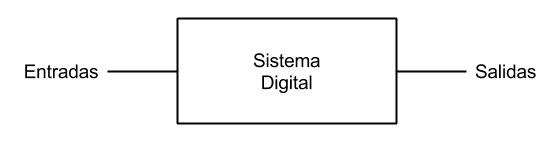
\includegraphics[width=2in]{sistemad}
\end{figure}

\end{frame}
%------------------------------------------------

\begin{frame}
\frametitle{Teorema de muestreo}

\begin{itemize}
\item Una señal limitada en banda de energia se puede recuperar de forma exacta a partir de sus muestras tomadas a una tasa de $f_{s}=2W$ muestras por segundo.
\end{itemize}

\begin{figure}[!h]
\centering
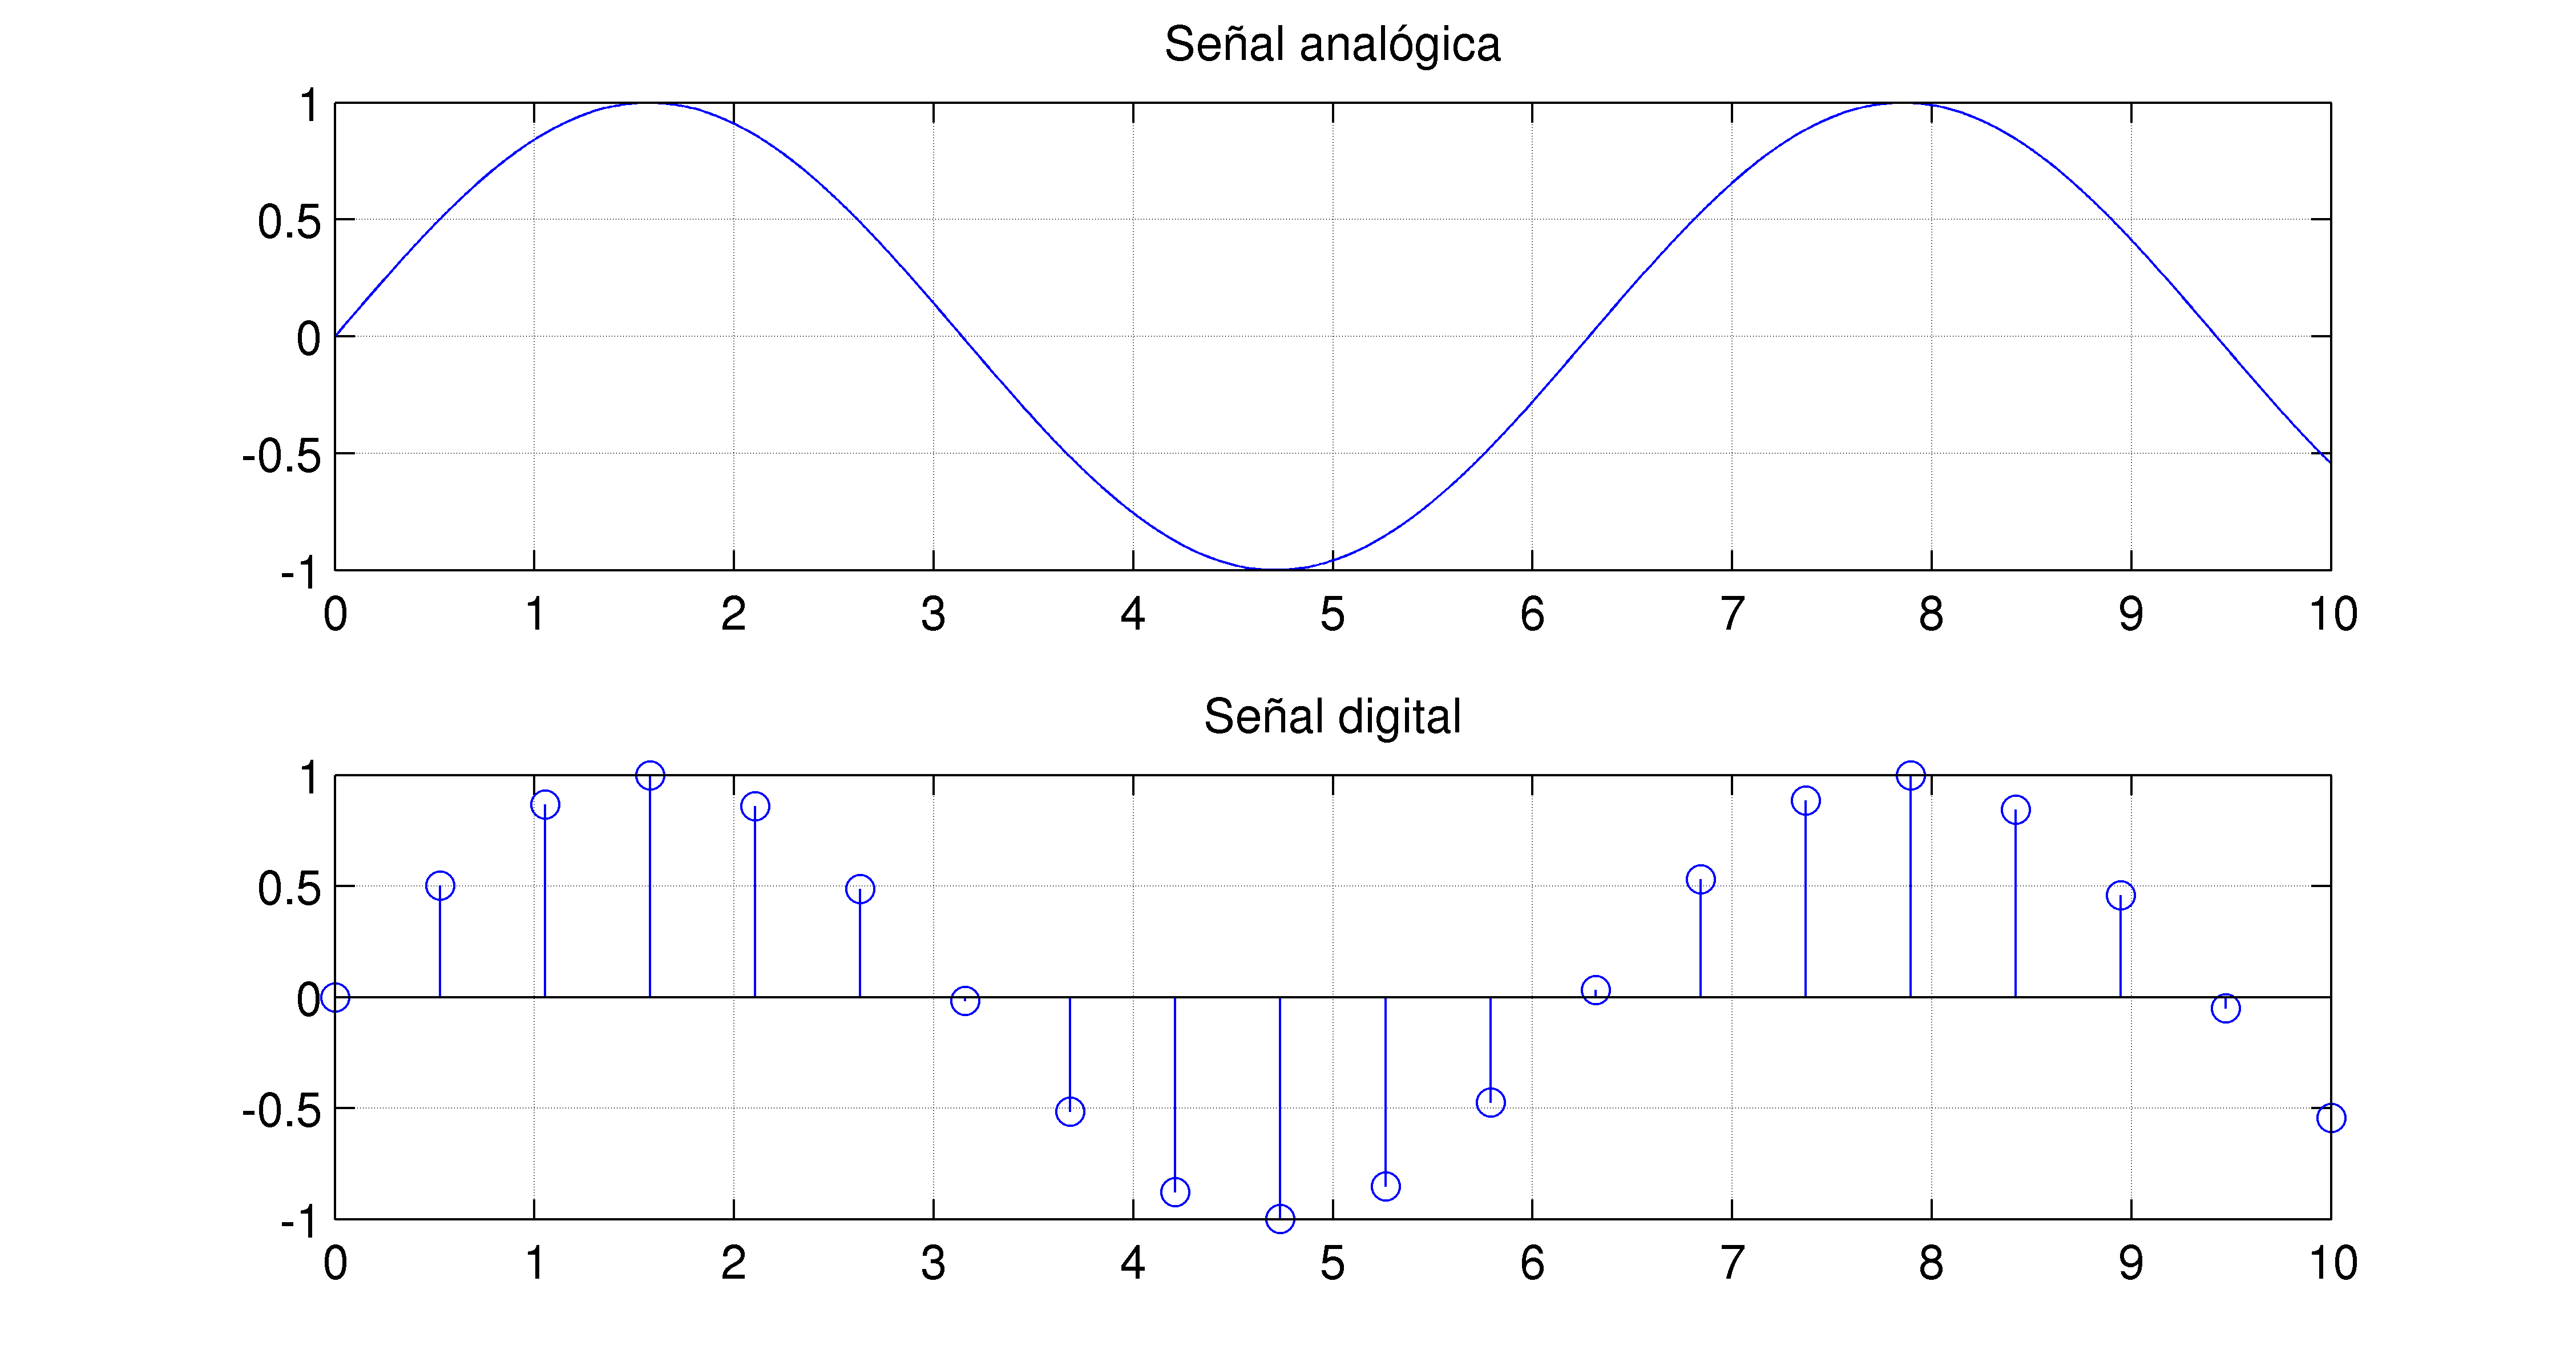
\includegraphics[width=4in]{muestreo}
\end{figure}

\end{frame}
%------------------------------------------------

\begin{frame}
\frametitle{Tensiones digitales}

\begin{itemize}
\item Las tensiones tienen solo dos valores: Alto (H) y Bajo (L).
\item Se producen cambios de una franja a la otra, llamados flancos.
\item Cuatro elementos principales: nivel alto, nivel bajo, flanco positivo o de subida y flanco negativo o de bajada.
\end{itemize}

\begin{figure}[!h]
\centering
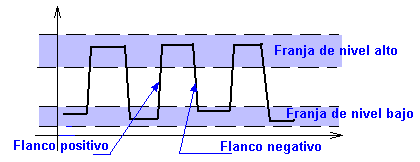
\includegraphics[width=3in]{tensionesd}
\end{figure}

\end{frame}
%------------------------------------------------

\section{Álgebra de Boole}

\begin{frame}
\frametitle{Postulados}

\begin{tabular}{c|c|c}
 & Suma & Producto \\ 
\hline 
Conmutativa & A+B=B+A & AB=BA \\ 
Asociativa & A+(B+C)=(A+B)+C & A(BC)=(AB)C \\ 
Distributiva & A+(BC)=(A+B)(A+C) & A(B+C)=(AB)+(AC) \\ 
Neutro & A+0=A & A*1=A \\ 
Complementario & A+$\overline{A}$=1 & A*$\overline{A}$=0 \\ 
\end{tabular} 

\end{frame}
%------------------------------------------------

\begin{frame}
\frametitle{Teoremas}
\begin{tabular}{c|c|c}
 & Suma & Producto \\ 
\hline 
Idempotencia & A+A=A & A*A=A \\ 
			 & A+1=1 & A*0=0 \\ 
Absorcion & A+(A*B)=A & A*(A+B)=A \\ 
De Morgan & $\overline{(A+B)}=\overline{A}*\overline{B}$ & $\overline{(A*B)}=\overline{A}+\overline{B}$ \\ 
Doble negacion & $\overline{(\overline{A})}=A$ & $\overline{(\overline{A})}=A$ \\ 
 & A+($\overline{A}$*B)=A+B & A*($\overline{A}$+B)=A*B \\ 
 & (AB)+(A$\overline{B}$)=A & (A+B)*(A+$\overline{B}$)=A \\ 
\end{tabular} 
\end{frame}
%------------------------------------------------

\section{Compuertas}

\begin{frame}
\frametitle{Compuerta AND}
\begin{columns}[c]
\column{.5\textwidth}
\begin{center}
\begin{tabular}{cc|c}
A & B & Q \\ 
\hline 
0 & 0 & 0 \\  
0 & 1 & 0 \\  
1 & 0 & 0 \\ 
1 & 1 & 1 \\ 
\end{tabular} 
\end{center}
\column{.5\textwidth}
\begin{figure}[!h]
\centering
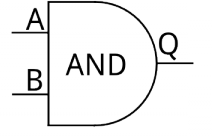
\includegraphics[width=1.5in]{and}
\end{figure}
\end{columns}
\end{frame}
%------------------------------------------------

\begin{frame}
\frametitle{Compuerta OR}
\begin{columns}[c]
\column{.5\textwidth}
\begin{center}
\begin{tabular}{cc|c}
A & B & Q \\ 
\hline 
0 & 0 & 0 \\  
0 & 1 & 1 \\  
1 & 0 & 1 \\ 
1 & 1 & 1 \\ 
\end{tabular} 
\end{center}
\column{.5\textwidth}
\begin{figure}[!h]
\centering
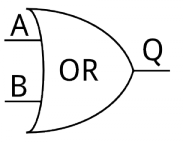
\includegraphics[width=1.5in]{or}
\end{figure}
\end{columns}
\end{frame}
%------------------------------------------------

\begin{frame}
\frametitle{Compuerta NOT}
\begin{columns}[c]
\column{.5\textwidth}
\begin{center}
\begin{tabular}{c|c}
A & Q \\ 
\hline 
0 & 1 \\   
1 & 0 \\ 
\end{tabular} 
\end{center}
\column{.5\textwidth}
\begin{figure}[!h]
\centering
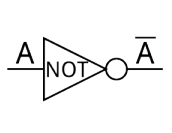
\includegraphics[width=1.5in]{not}
\end{figure}
\end{columns}
\end{frame}
%------------------------------------------------

\begin{frame}
\frametitle{Compuerta NAND}
\begin{columns}[c]
\column{.5\textwidth}
\begin{center}
\begin{tabular}{cc|c}
A & B & Q \\ 
\hline 
0 & 0 & 1 \\  
0 & 1 & 1 \\  
1 & 0 & 1 \\ 
1 & 1 & 0 \\ 
\end{tabular} 
\end{center}
\column{.5\textwidth}
\begin{figure}[!h]
\centering
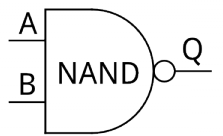
\includegraphics[width=1.5in]{nand}
\end{figure}
\end{columns}
\end{frame}
%------------------------------------------------

\begin{frame}
\frametitle{Compuerta NOR}
\begin{columns}[c]
\column{.5\textwidth}
\begin{center}
\begin{tabular}{cc|c}
A & B & Q \\ 
\hline 
0 & 0 & 1 \\  
0 & 1 & 0 \\  
1 & 0 & 0 \\ 
1 & 1 & 0 \\ 
\end{tabular} 
\end{center}
\column{.5\textwidth}
\begin{figure}[!h]
\centering
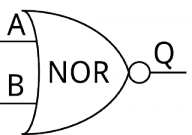
\includegraphics[width=1.5in]{nor}
\end{figure}
\end{columns}
\end{frame}
%------------------------------------------------

\begin{frame}
\frametitle{Compuerta XOR}
\begin{columns}[c]
\column{.5\textwidth}
\begin{center}
\begin{tabular}{cc|c}
A & B & Q \\ 
\hline 
0 & 0 & 0 \\  
0 & 1 & 1 \\  
1 & 0 & 1 \\ 
1 & 1 & 0 \\ 
\end{tabular} 
\end{center}
\column{.5\textwidth}
\begin{figure}[!h]
\centering
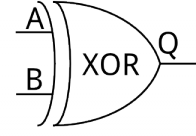
\includegraphics[width=1.5in]{xor}
\end{figure}
\end{columns}
\end{frame}
%------------------------------------------------

\begin{frame}
\frametitle{Escalas de integración}
Es una clasificación por el número de transistores que han sido fabricados dentro de un circuito integrado. Las clases son:
\vspace{0.4in}

\begin{tabular}{|c|c|c|}
\hline 
\textbf{Nombre} & \textbf{Significado} & \textbf{Transistores} \\ 
\hline 
SSI & Pequeña escala de integración & $<$50 \\ 
\hline 
MSI & Media escala de integración & 50-500 \\ 
\hline 
LSI & Larga escala de integración & 500-50000 \\ 
\hline 
VLSI & Muy larga escala de integración & 50000-500000 \\ 
\hline 
ULSI & Ultra larga escala de integración & $>$500000 \\ 
\hline 
\end{tabular} 

\end{frame}
%------------------------------------------------


\section{Logica combinacional}

\begin{frame}
\frametitle{Analisis de circuitos combinacionales}
\begin{columns}[c]
\column{.5\textwidth}
\begin{circuitikz} \draw
(0,2) node[and port] (myand) {}
(2,1) node[nor port] (mynor) {}
(myand.in 1) node[anchor=east] {C}
(myand.in 2) node[anchor=east] (bnode) {B}
(myand.out) -| (mynor.in 1)
node[below=of bnode] (cnode) {A}
(cnode) -| (mynor.in 2)
;\end{circuitikz}

$$f = \overline{(C \times B) + A}$$

\column{.5\textwidth}

Tabla de verdad: $2^{n}$, n=entradas

\vspace{0.2in}
\begin{tabular}{ccc|c}
C & B & A & f \\ 
\hline 
0 & 0 & 0 & 1 \\ 
0 & 0 & 1 & 0 \\ 
0 & 1 & 0 & 1 \\
0 & 1 & 1 & 0 \\ 
1 & 0 & 0 & 1 \\ 
1 & 0 & 1 & 0 \\ 
1 & 1 & 0 & 0 \\ 
1 & 1 & 1 & 0 \\ 
\end{tabular}
\end{columns}
\end{frame}
%------------------------------------------------

\begin{frame}
\frametitle{Simplificacion de circuitos combinacionales}
\begin{columns}[c]
\column{.5\textwidth}
Suma de productos (SOP)
\begin{Karnaughvuit}
   \minterms{0,2,4}
   \maxterms{1,3,5,6,7}
   %\indeterminats{2,5}
   \implicantcostats{0}{2}
   \implicant{0}{4}
\end{Karnaughvuit}
$$f_{SOP} = (\overline{C}*\overline{A}) + (\overline{B}*\overline{A})$$
\column{.5\textwidth}
Producto de sumas (POS)
\begin{Karnaughvuit}
   \minterms{0,2,4}
   \maxterms{1,3,5,6,7}
   %\indeterminats{2,5}
   \implicant{1}{7}
   \implicant{7}{6}
\end{Karnaughvuit}
$$f_{POS} = \overline{A}*(\overline{C}+\overline{B})$$
\end{columns}
\end{frame}
%------------------------------------------------

\section{Logica secuencial}

\begin{frame}
\frametitle{Circuito secuencial}
\begin{itemize}
\item Hasta ahora solo hemos visto los circuitos combinacionales, cuyas salidas dependen exclusivamente de las entradas.
\item Sin embargo, en los sistemas digitales, es indispensable el poder contar con memoria o bien, con estados internos. De esta manera se puede actuar en base a la historia.
\item En general, un circuito secuencial esta compuesto por circuitos combinacionales y elementos de memoria. Se dice que en un circuito secuencial la salida actual depende de la entrada actual y del estado actual del circuito.
\end{itemize}
\end{frame}
%------------------------------------------------

\begin{frame}
\frametitle{Circuito secuencial}
\begin{figure}[!h]
\centering
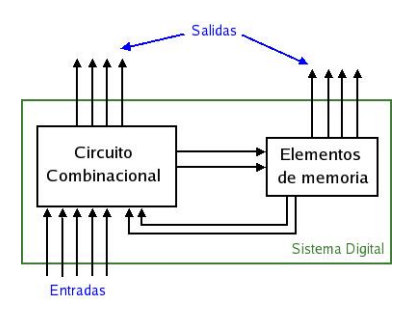
\includegraphics[width=3in]{secuencial}
\end{figure}
\end{frame}
%------------------------------------------------

\begin{frame}
\frametitle{Contador de 4 bits sincrónico con FF JK}

\begin{center}
\begin{tikzpicture}[scale=0.9]
    % Place the JK-Flip-Flops
  \JKFF(0,0){a}{$Q_0$}
  \JKFF(2,0){b}{$Q_1$}
  \JKFF(5.5,0){c}{$Q_2$}
  \JKFF(9,0){d}{$Q_3$}
  % Connect all the K and J ports
  \draw (a K) to[short,-*] (a J);
  \draw (b K) to[short,-*] (b J);
  \draw (c K) to[short,-*] (c J);
  \draw (d K) to[short,-*] (d J);
  % Connect the T ports to the incoming signal
  \draw (-1,-1) node[ocirc,label={left:$CLK$}] (CLK) {};
  \draw (a T) -- ++(-0.2,0) coordinate (inter) -|
    (CLK -| inter) node[circ] {};
  \draw (b T) -- ++(-0.2,0) coordinate (inter) -|
    (CLK -| inter) node[circ] {};
  \draw (c T) -- ++(-0.2,0) coordinate (inter) -|
    (CLK -| inter) node[circ] {};
  \draw (d T) -- ++(-0.2,0) coordinate (inter) -|
    (CLK -| inter) node[circ] {} -- (CLK);
  % Place the bits and the +
  \draw[->] (a J) -- ++(0,1) node[left] {$+$};
  \draw (a Q) to[short] ++(0,2) node[ocirc,label={left:Bit 0}] (bit0) {};
  \draw (b Q) to[short] ++(0,2) node[ocirc,label={left:Bit 1}] (bit1) {};
  \draw (c Q) to[short] ++(0,2) node[ocirc,label={left:Bit 2}] (bit2) {};
  \draw (d Q) to[short] ++(0,2) node[ocirc,label={left:Bit 3}] (bit3) {};
  % AND ports
  \draw (c J) |- ++(-0.2,0.5) node[and port] (c and) {};
  \draw (d J) |- ++(-0.2,1.5) node[and port] (d and) {};
  % Output connections
  \draw (b J) to[short,-*] (a Q);
  \draw (c and.in 2) to[short,-*] (c and.in 2 -| bit1);
  \draw (c and.in 1) to[short,-*] (c and.in 1 -| bit0);
  \draw (d and.in 2) to[short,-*] (d and.in 2 -| bit2);
  \draw (d and.in 1) to[short,-*] (d and.in 1 -| bit0);
  % I had to guess this connection, because the and port doesn't
  % have additional anchors
  \draw ($(d and.in 2)!0.5!(d and.in 1)+(0.4,0)$) coordinate (help)
    to[short,-*] (help -| bit1);
\end{tikzpicture}
\end{center}

\end{frame}
%------------------------------------------------

\begin{frame}
\frametitle{Forma de onda en el tiempo}
\begin{figure}[!h]
\centering
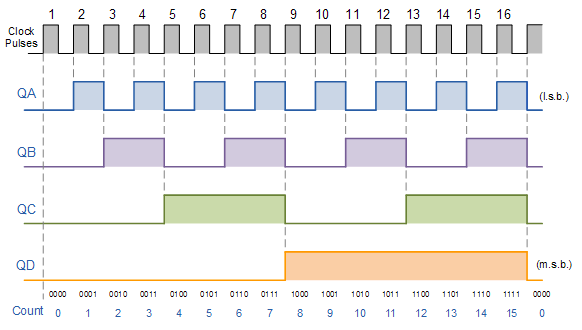
\includegraphics[width=4in]{waveform}
\end{figure}
\end{frame}
%------------------------------------------------

\begin{frame}
\frametitle{Explicación}

\begin{itemize}
\item Se puede observar que los pulsos de reloj alimentan directamente a cada uno de los FF JK en cadena y que tanto las entradas J y K están unidas entre sí en modo de conmutación.

\item Las entradas J y K del FFB están conectados directamente a la salida de control de calidad del FFA, pero las entradas J y K del FFC y FFD se alimentan con las señales de la entrada y salida de la etapa anterior. Esto genera la lógica requerida para las entradas JK de la siguiente etapa.

\item A continuación, ya que no hay retardo de propagación inherente en contadores sincrónicos, porque todas las etapas contadoras se activan en paralelo al mismo tiempo, la frecuencia máxima de funcionamiento de este tipo de contador sera mayor que la de un circuito contador asíncrono similar.
\end{itemize}

\end{frame}
%------------------------------------------------

\end{document}